% Chapter 2

\chapter{Theory and Motivation} % Chapter title

\label{ch:theory} % For referencing the chapter elsewhere, use \autoref{ch:examples} 
The \ac{SM} of particle physics represents all particles and interactions currently understood by the particle physics community. It is formulated using the principles of Quantum Field Theory, with the constraints of several symmetries and physical requirements to determine the rules for allowed interactions. \cite{Burgess:2007zi} Developed in the 1960s and 70s, it has been immensely successful at predicting additional particles, and has held up to many high-precision tests. Despite this success, it has several shortcomings which point to its incompleteness. Though the \ac{SM} is likely correct at the energies thus far probed, it may be missing key components that become more important at higher energies. Models supplementing the \ac{SM} with additional particles and interactions are referred to as \ac{BSM} theories. 

One possible extension of the \ac{SM} is \ac{SUSY}, a theory which applies an additional symmetry between bosons and fermions to the \ac{SM}, creating a spectrum of \ac{SUSY} particles (sparticles) which interact with the particles of the \ac{SM}. This theory motivates the search performed in \autoref{part:search}, and its theoretical appeals are discussed in this section, along with specific simplified models considered in the search. 

%----------------------------------------------------------------------------------------

\section{The Standard Model}
\label{sec:standard_model}
The \ac{SM} of particle physics describes the interactions of all of the particles currently known to exist, and consists of both matter particles and force carriers. This model has been unprecedentedly successful in predicting new particles and phenomena, including the prediction of the Higgs particle almost 50 years before its discovery in 2012, which completed the \ac{SM}. This section describes the components of the \ac{SM} and how they interact, focusing on the environment of the \ac{LHC}. 

The particles of the \ac{SM} are divided into two categories: fermions and bosons. The fermions comprise all the matter described by the \ac{SM}, and are spin-$\frac{1}{2}$ particles. The bosons, integer-spin particles, are the force carriers. They provide a mechanism to explain three of the four forces known to particle physics, with gravity still lacking a quantum formalization. The Higgs boson, the only spin-0 particle in the \ac{SM}, provides a mechanism for giving mass to the other particles. The full \ac{SM}, with the addition of the hypothetical graviton, is presented in \autoref{fig:sm}. 

\begin{centering}
\begin{figure}[bth]
\myfloatalign
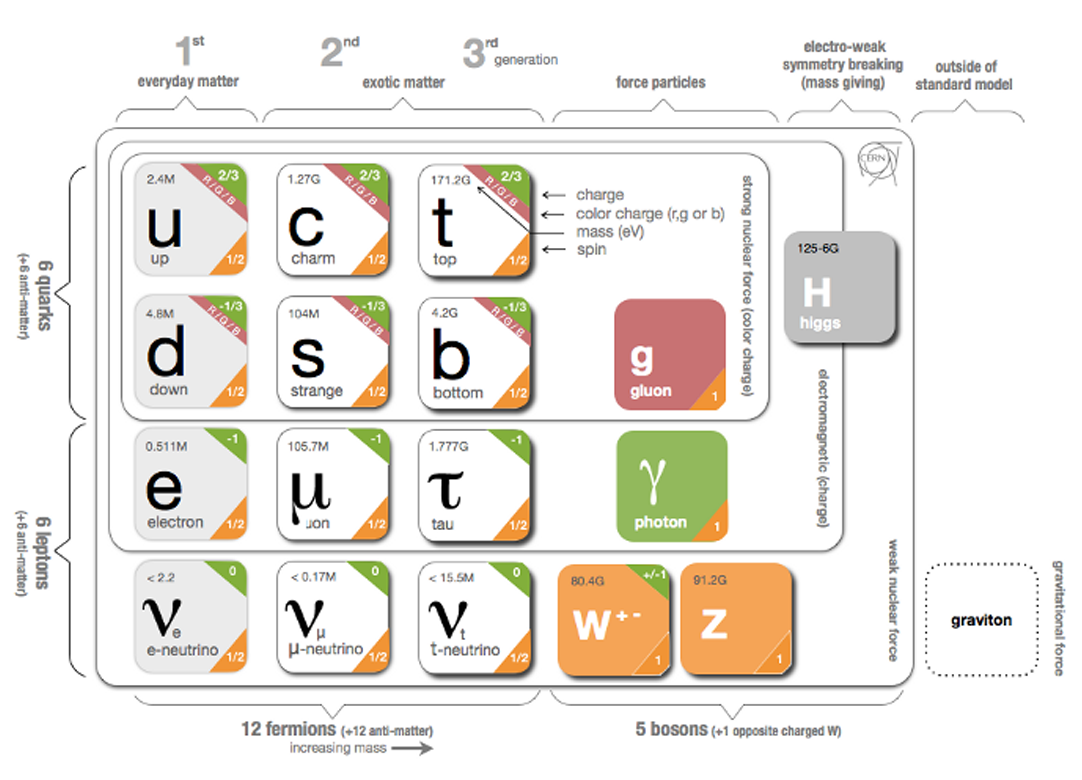
\includegraphics[width=.85\linewidth]{figures/theory/standardmodel.png}
\caption{The Standard Model of particle physics, containing all known bosons and fermions, with the addition of the hypothetical graviton. \cite{Galbraith:2012}}
\label{fig:sm}
\end{figure}
\end{centering}

\subsection{Matter}
\label{sec:matter}

The matter described by the \ac{SM} is made up of fermions, spin-$\frac{1}{2}$ particles which can be broken into two groups, quarks and leptons. The leptons all interact weakly, while the quarks additionally interact strongly. 

\subsubsection{Leptons}

Leptons, as seen in the bottom left of \autoref{fig:sm}, come in three generations, each labeled by a flavor: electron, muon, and tau. In the case of the massive leptons, these flavors are mass eigenstates, and the generations are placed in an order based on increasing mass. Each massive lepton is negatively charged and has a positively charged anti-particle. 

The three neutrinos come in the same flavors as the massive leptons, but these flavor eigenstates do not correspond exactly to mass eigenstates. As a consequence, neutrinos oscillate between flavors as they propagate through space. These oscillations are the only evidence of neutrino mass, which is bound from below by the mass splittings determined from the oscillation. Though it is still uncertain if the masses of the neutrinos follow the same hierarchy as the massive leptons, that expected ordering is slightly preferred over the inverted hierarchy. \cite{Huang:2016} 

Unlike the massive leptons, the neutrinos are uncharged, and it is not yet known whether each neutrino has a separate anti-particle, or if it is its own antiparticle. Because they are uncharged, they can only interact weakly, making them extremely difficult to detect. In the ATLAS detector, neutrinos pass through all layers undetected, and their presence can only be inferred from the non-conservation of momentum that results in the observed particles. As a consequence of their ability to evade detection, neutrinos are the least understood particles of the \ac{SM}. 

The \ac{SM} conserves lepton number, $L$, which is defined as the number of leptons minus the number of anti-leptons in a state. While this conservation is not theoretically required, its violation has not yet been observed. As a consequence of this conservation, the lightest massive lepton, the electron, is stable.

\subsubsection{Quarks}
\label{sec:quarks}

Quarks, as seen in the top left of \autoref{fig:sm}, are also charged particles that interact weakly, but are differentiated from the leptons by their strong interactions. They are also organized in three generations ordered by mass, and come in pairs of ``up-type'' and ``down-type'' quarks, named after the lightest generation. Though the up quark is lighter than the down, that rule is reversed in the subsequent two generations. Up-type quarks are charged $+\frac{2}{3}$, while the down-type quarks are charged $-\frac{1}{3}$. Quarks are also charged under the strong interaction, whose three charges are often characterized by colors: red, green, and blue. Each quark has an anti-particle with the opposite charges. 

These fractional charges and individual colors are never seen in nature because of the requirement (discussed further in \autoref{sec:strong}) that stable particle states be color-neutral. To accomplish this, quarks can create two-particle bound states called \textit{mesons} consisting of one quark and one anti-quark with the same color charge or three-particle bound states of quarks or anti-quarks with the three different color charges, which are called \textit{baryons}. The lightest color neutral state containing only quarks, the proton ($uud$), is stable. Extremely unstable bound states consisting of higher numbers of quarks can also exist, such as the pentaquark discovered in 2015 at the \ac{LHC}. \cite{Pentaquark} Collectively, these multi-quark bound states are called \textit{hadrons}. 

Like leptons, the number of quarks in a state is conserved. However, because quarks cannot exist in an isolated state, that conservation described as a conservation of baryon number ($B$) defined similarly to lepton number. Mesons, because they have one quark and one anti-quark, have $B = 0$. 

\subsection{Forces}

The fermions in the previous section interact via the electromagnetic, weak, and strong forces. In a perturbative quantum field theory, interactions via these forces are represented by mediating bosons. These force carriers interact only with particles charged with their  force's quantum numbers. The photon, for example, interacts only with electromagnetically charged particles. Gluons, mediators of the strong force, interact only with color charged particles, quarks and gluons. All fermions are weakly charged and interact with the weak force's mediators, the $W$ and $Z$ bosons. 

The formulation for each of these forces is developed by requiring that the \ac{SM} lagrangian be locally gauge invariant. \cite{Griffiths:111880} This can be accomplished by adding gauge fields to the lagrangian, whose behavior under gauge transformations cancels out the gauge dependence of the free lagrangian. However, adding a mass term for these fields reintroduces gauge dependence, so this mechanism only creates forces mediated by massless gauge bosons. The addition of the Higgs field provides mass terms the weak gauge bosons without interfering with the gauge invariance. 

The total gauged symmetry group for the \ac{SM} is $SU_c(3) \times SU_L(2) \times U_Y(1)$, with a total lagrangian which can be divided into several terms

\begin{equation}
\mathcal{L}_{SM} = \mathcal{L}_{strong} + \mathcal{L}_{electroweak}
\end{equation}

each of which will be described in detail in their respective sections. 

\subsubsection{The Electromagnetic Force}
\label{sec:em}

The simplest example of gauge invariance requirements generating a description of a force can be found in electromagnetism. It has one massless mediator, the photon, which interacts with all electromagnetically charged particles. What follows is a brief description of how enforcing this invariance generates a lagrangian of the same form as the classical electromagnetic lagrangian, which can be easily incorporated into the \ac{SM}. 

The particles in ~\autoref{sec:matter} are fermions, and so their free lagrangians are Dirac lagrangians and all follow the form

\begin{equation}
\mathcal{L} = i\bar{\psi}\gamma^\mu \partial_\mu\psi - m \bar{\psi}\psi . 
\end{equation}

Requiring that the free lagrangians for these particles be invariant under a $U(1)$ local gauge transformation, $e^{iq\lambda(x)}$, can be accomplished by adding a term to the lagrangian which cancels the derivative term arising from $\lambda$'s dependence on $x$: 

\begin{equation}
\mathcal{L} = i\bar{\psi}\gamma^\mu \partial_\mu\psi - m \bar{\psi}\psi - (q\bar{\psi}\gamma^\mu\psi)A_\mu
\end{equation}

where $A_\mu$ is a ``gauge field'' that transforms according to 

\begin{equation}
A_\mu \rightarrow A_\mu + \partial_\mu \lambda . 
\end{equation}

This vector field must also come with a free term, 

\begin{equation}
\mathcal{L} = -\frac{1}{16\pi}F^{\mu\nu}F_{\mu\nu} + \frac{1}{8\pi}m_A^2A^\nu A_\nu . 
\end{equation}

The mass term for this field would not itself be invariant under the transformation, but the field can simply be made massless to avoid this problem. The final lagrangian, then, is 

\begin{equation}
\mathcal{L} = i\bar{\psi}\gamma^\mu \partial_\mu\psi - m \bar{\psi}\psi -\frac{1}{16\pi}F^{\mu\nu}F_{\mu\nu} - (q\bar{\psi}\gamma^\mu\psi)A_\mu
\label{eq:l_em}
\end{equation}

which is precisely the original lagrangian with the addition of terms replicating the form of the Maxwell lagrangian. In a quantized interpretation, it describes a field that interacts with particles with non-zero electromagnetic charge $q$ via interactions with a massless spin-1 boson, the photon. 

For the purpose of succinct notation, this lagrangian is often rewritten in terms of the ``covariant derivative''

\begin{equation}
\mathcal{D}_\mu = \partial_\mu + iq\lambda A_\mu
\end{equation}

which immediately cancels the gauge dependent term created by the transformation. This mechanism is mathematically simple in the $U(1)$ case, but can be replicated for more complicated gauge transformations with perturbative approximations. 

%-------------------------------------------------------------------------------------------------------

\subsubsection{The Strong Force}
\label{sec:strong}

The strong force is generated by a similar process of requiring local gauge invariance, but in this case, for a $SU(3)$ transformation. The interactions of the strong force are described by the theory of quantum chromodynamics, which is given by the lagrangian

\begin{equation}
\mathcal{L}_{strong} = -\frac{1}{4}G^\alpha_{\mu\nu}G^{\alpha\mu\nu} - \frac{1}{2}\bar{Q}_m \slashed{D} Q_m
\end{equation}

where the $\alpha$ index runs from 1 to 8 and represents the different generators of SU(3), and $m$ indexes the three quark generations. $G^\alpha_{\mu\nu}$ is the field strength tensor and is defined as

\begin{equation}
G^\alpha_{\mu\nu} = \partial_\mu G^\alpha_\nu - \partial_\nu G^\alpha_\mu + g_3 f^\alpha_{\beta\gamma}G^\beta_\mu G^\gamma_\nu
\end{equation}

where $g_3$ is a function of the energy scale of the interaction $\mu$, and is related to the strong coupling constant by

\begin{equation}
\alpha_s(\mu) =  g_s(\mu)^2 / 4\pi . 
\end{equation}

This first term of the lagrangian gives the gluon self-coupling interactions, with terms involving 2, 3, and 4 gluon field terms. The 2-field portion is simply the field strength tensor, but the other terms give couplings that can be described by the feynman diagrams in \autoref{fig:feynman_gluons}.

\begin{centering}
\begin{figure}[!hbt]
\myfloatalign
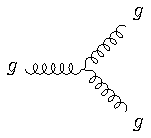
\includegraphics[width=.45\linewidth]{feynman/gluon_3.pdf}
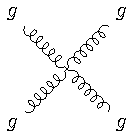
\includegraphics[width=.4\linewidth]{feynman/gluon_4.pdf}
\caption{Gluon self coupling Feynman diagrams involving 3- and 4-gluon interactions.}
\label{fig:feynman_gluons}
\end{figure}
\end{centering}

In the second term, $\slashed{D} Q_m$ is the covariant derivative acting on the quark field. The quarks are in fact charged under all three forces, strong, electromagnetic, and weak, so the covariant derivative includes terms to make each of the force's lagrangians gauge invariant. Thus this term introduces quark-boson interactions of four types, seen in \autoref{fig:feynman_quarks}. The quarks' coupling to the gluon is the strongest, with the other couplings happening at lower rates. The couplings to the $W$ and $Z$ bosons will be described in \autoref{sec:ew}.

\begin{centering}
\begin{figure}[!hbt]
\myfloatalign
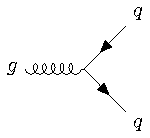
\includegraphics[width=.45\linewidth]{feynman/quark_strong.pdf}
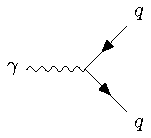
\includegraphics[width=.45\linewidth]{feynman/quark_em.pdf}
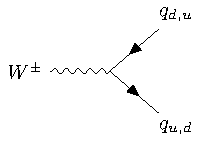
\includegraphics[width=.45\linewidth]{feynman/quark_w.pdf}
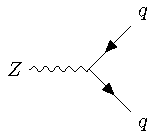
\includegraphics[width=.45\linewidth]{feynman/quark_z.pdf}
\caption{Quark couplings to the different types of gauge bosons. The $q_{u,d}$ labels represent any up- or down-type quarks.}
\label{fig:feynman_quarks}
\end{figure}
\end{centering}

The canceling required to make the lagrangian gauge invariant is actually only satisfied to a first order expansion of the transformation, guaranteeing its validity only for infinitesimally small perturbations from the ground state. However, the strong coupling constant, $\alpha$, depends on the energy scale of the interaction, decreasing at higher energy scales and asymptotically increasing at low energies. \autoref{fig:alpha} shows this effect translated to distance scales, demonstrating that QCD is weak and can be considered perturbatively at small distance scales, but at large distance scales this approximation breaks down, and the colorless hadrons introduce in ~\autoref{sec:quarks} must be used to describe interactions instead. 

\begin{centering}
\begin{figure}[bth]
\myfloatalign
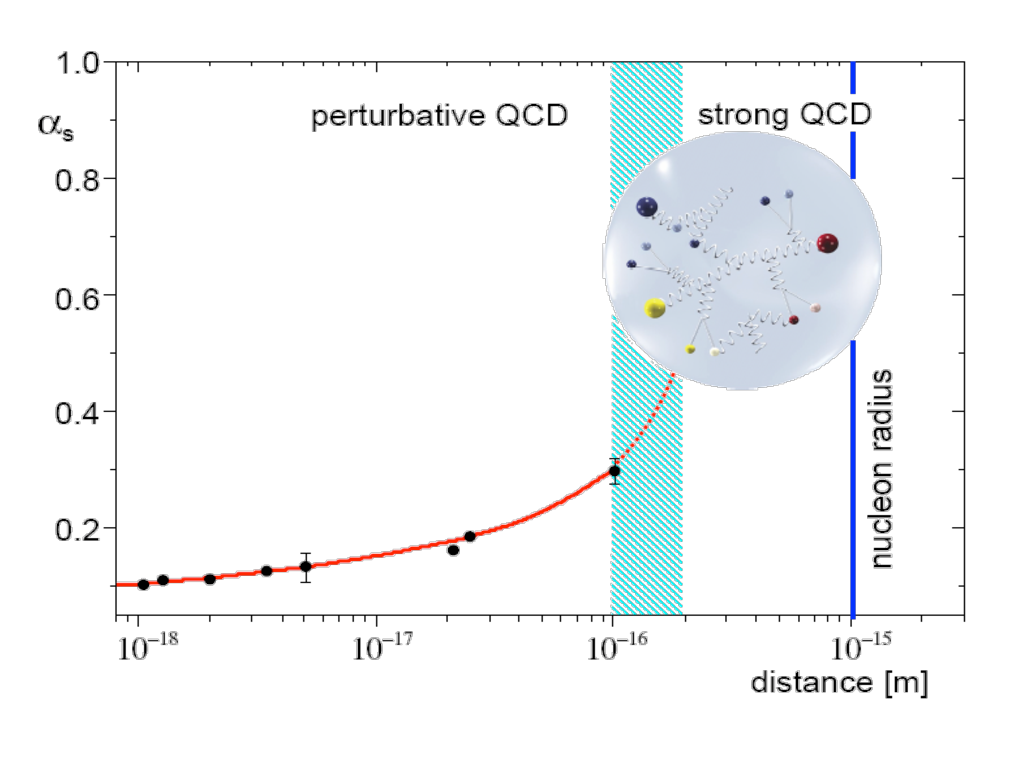
\includegraphics[width=.85\linewidth]{figures/theory/strong_coupling.png}
\caption{The running of the strong coupling constant, $\alpha_s$. \cite{Messchendorp:2013ysj}}
\label{fig:alpha}
\end{figure}
\end{centering}

The boundary between these regimes is referred to as $\Lambda_{QCD}$ and differentiates energies at which quarks can be considered free particles and the energies at which they must instead be described by their colorless bound states. The \ac{LHC} is capable of producing individual quarks, but they instantaneously hadronize, producing showers of colored particles referred to as ``jets''. 


% \subsubsection{Quantum Chromodynamics}
% \label{sec:strong}

% \ac{QCD}, the theory describing the strong force, can be formulated similarly to the electromagnetic force, but with a $SU(3)$ transformation replacing $U(1)$. This transformation acts on a vector of equal mass quarks, the three different colors of a given flavor. The transformation is written as follows,

% \begin{equation}
% \bm{\psi} \rightarrow e^{-iq\bm{\lambda}\cdot\bm{\phi}(x)}\bm{\psi}
% \end{equation}

% where $\bm{\phi}$ gives a vector of coefficients to be multiplied by the Gell-Man matrices, $\bm{\lambda}$. Though the math is more complicated than the $U(1)$ case in this higher dimensional rotation, the cancellation is ultimately similar. 

% The main difference, corresponding to this more complicated basis of transformations, is that eight fields $A_\mu$ are required rather than the one needed in electromagnetism. These eight fields correspond to eight massless bosons, the different color states of the gluon, the carrier of the strong force.  

% All together, the total lagrangian for \ac{QCD} is

% \begin{equation}
% \mathcal{L} = i\bar{\psi}\gamma^\mu \partial_\mu\psi - m \bar{\psi}\psi -\frac{1}{16\pi}\bm{F}^{\mu\nu}\bm{F}_{\mu\nu} - (q\bar{\psi}\gamma^\mu\psi)\bm{A}_\mu , 
% \end{equation}

% an equation identical in form to \autoref{eq:l_em}, with the mathematical complications of the additional fields hidden by the vector notation. In addition to that change, the covariant derivative must accommodate a vector $\bm{A}$ as well, changing only slightly to be defined as

% \begin{equation}
% \mathcal{D}_\mu = \partial_\mu + iq\bm{\lambda} \cdot \bm{A}_\mu .
% \end{equation}


\subsubsection{The Weak Force}
\label{sec:ew}

A similar process, using an $SU(2)$ gauge transformation, can produce a lagrangian that would suffice to describe the $W$ and $Z$ bosons of the \ac{SM}, if only they were massless. However, they are not, so an alternate mechanism must be used to add masses to the lagrangian. 

Before a mechanism for their masses was understood, and before they were discovered, the large mass of the $W$ and $Z$ bosons were proposed in order to unify the electromagnetic and weak forces into the electroweak force. The large masses were crucial to explain the discrepancy in the strength of the two forces. 

This unified theory resulted in a triplet, $\bm{W}$, with coupling $g_W$, and a singlet field $B$, with coupling $g'/2$. However, this electroweak symmetry is broken, and mixing between these states occurs. Rewritten in their mass basis, the more familiar electroweak force carriers are produced: $W^\pm$, two states with identical coupling resulting from the first two states of the $W$ triplet, then $Z^0$ and the photon field $A$ resulting from the mixing of the last $W$ state and $B$. 

The electroweak lagrangian is much more complicated than the strong lagrangian, and can be divided into several terms:

\begin{equation}
\mathcal{L}_{electroweak} = \mathcal{L}_{gauge} + \mathcal{L}_{fermions} + \mathcal{L}_{Higgs} + \mathcal{L}_{Yukawa} .
\end{equation}

The first term can be written as follows

\begin{equation}
\mathcal{L}_{gauge} = -\frac{1}{4}W^{a\mu\nu}W^a_{\mu\nu} - \frac{1}{4}B^{\mu\nu}B{\mu\nu} 
\end{equation}

where the $a$ indices are numbered 1 through 3 and indicate the generators of $SU(2)$ and is written 

\begin{equation}
W^\alpha_{\mu\nu} = \partial_\mu W^a_\nu - \partial_\nu W^a_\mu + g_2 \epsilon_{abc} W^b_\mu W^c_\nu
\end{equation}

The gauge portion of the lagrangian then generates interaction terms of between the three W fields, which when rewritten in terms of the mass-eigenstate basis, generates interactions like the ones in \autoref{fig:tlgc}.

\begin{centering}
\begin{figure}[!hbt]
\myfloatalign
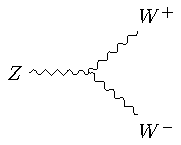
\includegraphics[width=.45\linewidth]{feynman/tlgc_z.pdf}
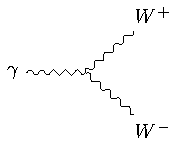
\includegraphics[width=.45\linewidth]{feynman/tlgc_g.pdf}
\caption{Trilinear gauge couplings in the \ac{SM}.}
\label{fig:tlgc}
\end{figure}
\end{centering}

The fermion portion of the lagrangian is written as

\begin{equation}
\begin{split}
\mathcal{L}_{fermion} = & -\frac{1}{2}\bar{L}_m\slashed{D}L_m -\frac{1}{2}\bar{Q}_m\slashed{D}Q_m \\
						& -\frac{1}{2}\bar{U}_m\slashed{D}U_m -\frac{1}{2}\bar{D}_m\slashed{D}D_m \\
						& -\frac{1}{2}\bar{E}_m\slashed{D}E_m \\
\end{split}
\end{equation}

with the inclusion of the quark term already mentioned in \autoref{sec:strong} for completeness. 
***** finish this with an explanation of handedness and and then draw feynman diagrams then move on to mass terms and into higgs mechanism. Figure out what to do with neutrino masses. Maybe make Higgs chapter a subsection called electroweak symmetry breaking. 


\subsubsection{The Higgs Mechanism}

The reason for this symmetry breaking has to do with the final piece of the \ac{SM}, the Higgs boson. The Higgs mechanism presents an alternate way to generate a mass term, through an unexpected route. It is a scalar field, with a lagrangian 

\begin{equation}
\mathcal{L} = \frac{1}{2}(\partial_\mu\phi)^*(\partial^\mu\phi) + \frac{1}{2}\mu^2\phi^*\phi - \frac{1}{4}\lambda^4(\phi^*\phi)^2
\end{equation}

where $\phi$ is a complex scalar field, $\phi = \phi_1 + i\phi_2$. This looks very similar to the standard scalar field, but the signs on the mass and interaction terms are reversed, giving a result that looks like an imaginary mass. However, this lagrangian differs from all previously considered lagrangians in that its ground state does not occur at $\phi = 0$. Because this is a perturbative theory, its validity only holds when expanded around the ground states, which must satisfy

\begin{equation}
\phi_1^2 + \phi_2^2 = - \frac{\mu}{\lambda} . 
\end{equation}

Rewriting the original lagrangian in terms of fields centered around ground states chosen to satisfy that condition results in a reasonable mass term. However, in an effect called ``spontaneous symmetry breaking'', the original $SO(2)$ rotational symmetry of the lagrangian is lost, resulting only in a $U(1)$ rotational symmetry; the lagrangian is invariant under a phase transformation.

As in \autoref{sec:em}, it is possible to make the lagrangian invariant under a local $U(1)$ transformation, $\phi \rightarrow e^{i\theta(x)\phi}$ by adding a massless gauge field $A^\mu$ and using the covariant derivative. Due to the many cross terms from the non-zero ground state, terms for the mass of one of the bosons as well as the gauge field appear, leaving only one massless boson. The massless boson, it turns out, can be completely removed from the theory via local $U(1)$ transformations, ultimately producing a theory with one massive scalar (the Higgs) and a massive gauge field. 


% The original lagrangian can be put in terms of $\eta$ and $\xsi$, defined as

% \begin{equation}
% \eta = \phi_1 \pm \frac{\mu}{\lambda}  ; \xsi = \phi_2
% \end{equation}

% to read

% \begin{equation}
% \mathcal{L} = \frac{1}{2}(\partial_\mu\eta)(\partial^\mu\eta) - \mu^2\eta^2 \pm \mu\lambda\eta^3 - \frac{1}{4}\lambda^2\eta^4 + \frac{1}{4}(\frac{\mu^2}{\lambda})^2 . 
% \end{equation}

% This lagrangian now has a reasonable mass term ($m = \sqrt{2}\mu$) and several interaction terms. However, it no longer shares a symmetry of the original lagrangian; though $\mathcal{L}$ is invariant under $\phi \rightarrow e^{i\theta}\phi$, it is not invariant under $\eta \rightarrow e^{i\theta}\eta$. This is referred to as spontaneous symmetry breaking. 

\subsection{Phenomenology of Proton-Proton Collisions}
\label{sec:pp_collisions}

As discussed in \autoref{ch:lhc}, the \ac{LHC} collides bunches of high-energy protons, and the interactions of these protons' constituent quarks produce the wide array of particles seen in the ATLAS detector. The \ac{LHC} typically cites its energy in terms of $\sqrt{S}$, the center of mass energy of protons in the two colliding beams. However, because the proton is not fundamental, this energy is divided among many particles that make up the proton. 

To first order, a proton consists of three quarks: two up quarks and one down quark. However, a real quantum mechanical system is much more chaotic, with other quarks popping into and out of existence and gluons flying between them. These additional quarks are called ``sea'' quarks. The particles inside the proton can have a wide range of energies depending on the internal dynamics at the moment of the collision. These cannot be predicted exactly, but probabalistic models called \acp{PDF} describe the likelihood of any given configuration. These models are determined using data from hard scattering experiments and give probabalistic estimates for how often a given type of particle appears with a fraction $x$ of the total proton energy, as seen in \autoref{fig:pdf}. 

\begin{centering}
\begin{figure}[bth]
\myfloatalign
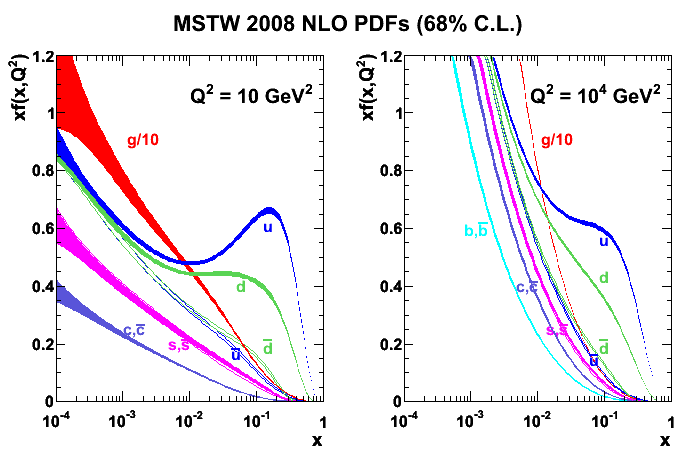
\includegraphics[width=.85\linewidth]{figures/theory/mstw2008nlo68cl_allpdfs.png}
\caption{2008 MSTW \acp{PDF} for various particle types. \cite{0901.0002}}
\label{fig:pdf}
\end{figure}
\end{centering}



%------------------------------------------------

\subsection{Problems in the Standard Model}
\label{sec:sm_problems}

Thought the \ac{SM} is a self-consistent theory that describes to great accuracy all of the particles and forces in includes, it does have certain shortcomings. The most glaring is the omission of gravity. Though the force is well understood at large scales via the theory of General Relativity, no satisfying quantum description of gravity has been accepted, much less proven. The Planck scale, the energy scale at which gravitational interactions become large enough that no sound theory can ignore gravity, is at about $10^28$ \eV,  16 orders of magnitude above the electroweak scale. 

Another clear omission of the \ac{SM} is \ac{DM}. This matter was first identified in 1933 through the observation of galactic rotation curves. \cite{zwicky} The speed of rotation indicated both that there was more mass in the system than could be accounted for by observations made directly of the galaxy, and that this additional matter was distributed in a halo, not a disk like the typical luminous matter. This effect can be seen in \autoref{fig:dm_curve}. Since then, the gravitational impact of \ac{DM} has been observed in colliding clusters and many more rotational curves, but it has never been directly detected or seen at a particle accelerator. As a consequence, very few details are known about the nature of the particles that make up this matter, only that it does not interact strongly or electromagnetically and its density throughout the universe. 

\begin{centering}
\begin{figure}[bth]
\myfloatalign
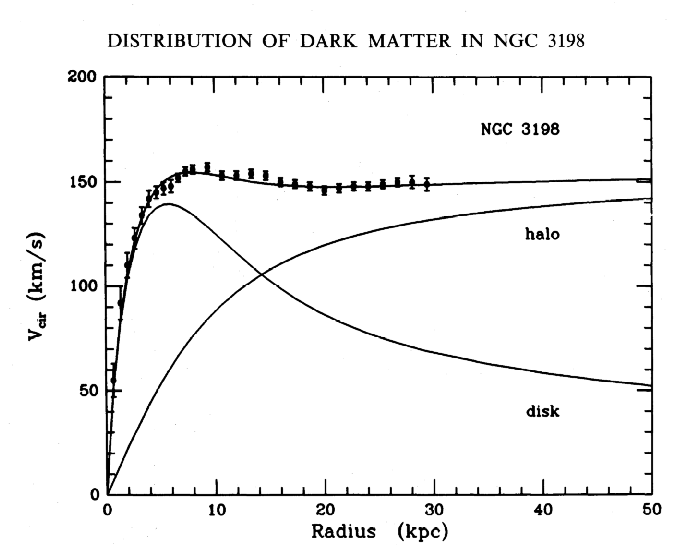
\includegraphics[width=.85\linewidth]{figures/theory/rotatioanl_curve_ngc3198_rc.png}
\caption{Galactic rotation curve showing that the discrepancy between the observed luminous matter and the total mass in the system can be described as a non-luminous halo of matter. \cite{1985ApJ...295..305V}}
\label{fig:dm_curve}
\end{figure}
\end{centering}

Beyond the omissions of the \ac{SM}, there are several aesthetic problems - things that could have no solution, but seem to suggest that the current \ac{SM} are missing some pieces that could unify it and provide more order. The first is the sheer number of parameters in the \ac{SM}. There are 26 independent parameters determining the mass of the particles and all the couplings between them. Besides the rough grouping of fermions into generations, there seems to be no order to masses of particles, and no way to predict the masses or couplings. Each, it seems, is independently provided by nature. 

In the past, large numbers of seemingly unrelated parameters has indicated that a theory has a more fundamental form at shorter distance scales. The large number of elements, it turned out, could be explained by different groupings of three particles, the proton, neutron and electron. Later, the menagerie of hadrons became so large that a similar reimagining of what was fundamental took place, and the theory of quarks gave an order to the many mesons and baryons. This pattern leaves physicists suspicious or any theory with too many particles and free parameters, suggesting that perhaps, at a higher energy, there is a simpler model that can unify many of the seemingly disparate elements of the \ac{SM}. 

However, some of these seemingly independent parameters have suspicious symmetry. The Higgs mass, for example, has been measured to be 125 \gev. This mass is the sum of the bare mass, the one that appears in the lagrangian, and quantum corrections from interactions with other particles, which are proportional to the square of the particles' mass. Since new physics must exist at the Planck scale to account for gravity, these corrections could be up to 35 orders of magnitude larger than the Higgs mass. The bare mass could theoretically cancel out this massive correction, these parameters should be independent, and the odds that they would be precisely the same to 35 places are very, very small. This exact canceling is often called ``fine-tuning'', an undesirable trait in a theory which suggests that some more fundamental symmetry has been missed. The word ``naturalness'' is used to describe the the extent to which a theory is free of fine-tuning. 

%-------------------------------------------------

\section{Supersymmetry}

\ac{SUSY} was proposed and developed in the 1970s to give solutions to many of these \ac{SM} shortcomings. The theory works by introducing a fermionic symmetry to the \ac{SM}, in addition to the usual spacetime symmetries of translations, rotations, and changes of Lorentz frame. The combination of the usual spacetime with this fermionic dimension is called a ``superspace''. Rotations in this dimension result in a particle's spin changing by 1/2, turning a spin-1/2 fermion into a spin-0 particle, for example. As a consequence, this symmetry requires the existence of many new particles - a bosonic ``sfermion'' for each fermion of the \ac{SM} and a fermionic ``gaugino'' for each of the gauge bosons. These superpartners of \ac{SM} particles should have identical quantum numbers to the original particle, except for their spin. \autoref{tab:sparticles} shows the \ac{SM} particles and their superpartners. 

%TODO make better figure

\begin{table}
\begin{center}
 \begin{tabular}{cc|c|c|c}
   \hline 
   \multicolumn{2}{c|}{Names} & sparticles & particles & $SU(3)_C, SU(2)_L, U(1)_Y$ \\
   \hline
   \hline
   \multirow{3}{*}{squarks, quarks} & $Q$ 		& ($\squ[L] \sqd[L]$) & ($u_L d_L$) 		& ($\bf{3}, \bf{2}, \frac{1}{6}$) 		\\
   									& $\squ$ 	& $\squ[R]^*$ 		& $u^\dagger_R$ 	& ($\bf{\bar{3}}, \bf{1}, -\frac{2}{3}$) 	\\
   									& $\sqd$ 	& $\sqd[R]^*$ 		& $d^\dagger_R$ 	& ($\bf{\bar{3}}, \bf{1}, \frac{1}{3}$) 	\\		
   \hline
   \multirow{2}{*}{sleptons, leptons} & $L$ 	& ($\slneu \sle[L]$) & ($\nu e_L$) 		& ($\bf{1}, \bf{2}, -\frac{1}{2}$) 		\\
   									& $\bar{e}$ & $\sle[R]^*$ 		& $e^\dagger_R$ 	& ($\bf{1}, \bf{1}, 1$) 					\\
   \hline
   \multirow{2}{*}{Higgs, higgsinos} & $H_u$ 	& ($\Hou[+] \Hou[0]$) 	& ($H^+_u H^0_u$)  & ($\bf{1}, \bf{2}, \frac{1}{2}$) 	\\
   									& $H_d$ 	& ($\Hod[0] \Hod[-]$) 	& ($H^0_d H^-_d$)  & ($\bf{1}, \bf{2}, -\frac{1}{2}$) 	\\  
   \hline
   \multicolumn{2}{c|}{gluino, gluon}	& $\go$ 			& $g$			& ($\bf{8}, \bf{1}, 0$)		\\							
   \hline
   \multicolumn{2}{c|}{winos, $W$ bosons}	& $\Wo^\pm \Wo^0$ 	& $W^\pm W^0$	& ($\bf{1}, \bf{3}, 0$)		\\							
   \hline
   \multicolumn{2}{c|}{bino, $B$ boson}	& $\Bo^0$ 			& $B^0$			& ($\bf{1}, \bf{1}, 0$)		\\							

\hline
\hline
 \end{tabular}
\end{center}
 \caption{Supermultiplets of the \ac{MSSM}. Sfermions, on the first five rows, are all spin-0. Higgsinos and gauginos are all spin-1/2. Three sets of each fermion's supermultiplet exist, one for each generation. \cite{Martin:1997ns}}
 \label{tab:sparticles}
\end{table}





If the theory is symmetric under these fermionic rotations, these particle-sparticle pairs can be described by a single ``superfield'', which simultaneously describes the behavior of both \ac{SM} and \ac{SUSY} particles in the superspace. However, this completely symmetric behavior is untenable given basic observations of matter in the universe. For example, if there were a ``selectron'' (the superpartner of the electron, $\sle$), for example, with identical mass to the electron, it would have been detected long ago. In fact, such a particle would fundamentally change atomic structure, with the bosonic selectrons capable of piling into the ground state of an atom, and removing all the interesting valence-shell interactions of electrons that determine molecular structure. Thus, if \ac{SUSY} does exist, the symmetry must be broken, with much higher masses for the superpartners than the original \ac{SM} particles. 

\subsection{The Minimal Supersymmetric Standard Model}

The \ac{MSSM} was designed to be the simplest supersymmetric extension of the \ac{SM} that remains self consistent, and it results in the particles seen in \autoref{tab:sparticles}\cite{Martin:1997ns}. The formulation of the \ac{MSSM} begins by introducing a second Higgs doublet to account for the different masses of the sparticles. As with the \ac{SM} Higgs, electroweak symmetry breaking results in the loss of degrees of freedom, and only five states remain, the lightest of which, $h^0$, can be interpreted as the \ac{SM} Higgs already discovered. There are two remaining neutral states, $A^0$ and $H^0$, as well as two charged Higgses, $H^\pm$. 

The neutral Higgs states mix with the neutral gauge bosons, while the charged Higgs states mix with the charged gauge bosons, producing a series of states labeled only by their charge and the order of their masses. The neutral states, collectively called the neutralinos, are identified from lightest to heaviest, $\No[1], \No[2], \No[3],$ and $\No[4]$. The charged states, referred to as charginos, are similarly called $\Co[1]$ and $\Co[2]$.

The \ac{MSSM} introduces many new interactions between \ac{SM} particles and sparticles. Though these don't represent all possible interactions, a general rule is that any \ac{SM} vertex can have two interacting particles replaced with their sparticle equivalents, and this vertex will be part of the \ac{MSSM}. \autoref{fig:mssm_int} gives two examples of such vertices. 

\begin{centering}
\begin{figure}[!hbt]
\myfloatalign
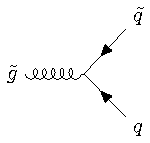
\includegraphics[width=.45\linewidth]{feynman/gluino.pdf}
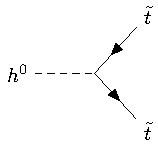
\includegraphics[width=.45\linewidth]{feynman/higgs_stop.pdf}
\caption{Two example vertices allowed by the \ac{MSSM}.}
\label{fig:mssm_int}
\end{figure}
\end{centering}

In addition to these interactions, there are several terms that appear in the \ac{MSSM} lagrangian that violate the $B$ and $L$ conservation conserved in the \ac{SM}. These superpotential terms appear as follows

\begin{eqnarray}
W_{\Delta L = 1} = \frac{1}{2}\lambda^{ijk}L_i L_j \bar{e}_k + \lambda'^{ijk}L_i Q_j \bar{d}_k + \mu'^i L_i H_u \\
W_{\Delta B = 1} = \frac{1}{2}\lambda''^{ijk}\bar{u}_i \bar{d}_j \bar{d}_k .
\label{eq:rviol}
\end{eqnarray}

Because there are very strong limits on non-conservation of $B-L$, the difference between baryon lepton number, from proton decay experiments, these terms present a challenge for the \ac{MSSM}. It would be possible, of course, to simply tune the $\lambda$ parameters to be small enough to fit within experimental constraints, but these terms can also be eliminated by introducing a new conserved quantity, $R$-parity. It is defined by

\begin{equation}
P_R = -1^{3(B-L)+2s}
\end{equation}

where $s$ is the spin of the particle. Requiring that all terms in the lagrangian have a multiplicative $P_R$ of 1 excludes the terms in \autoref{eq:rviol}, removing the problem of proton decay. All \ac{SM} particles are $R$-parity even, while the sparticles are $R$-parity odd. As a consequence, massive sparticles typically decay through a chain of lighter sparticles, emitting \ac{SM} particles along the way.  

\subsection{Solutions to Standard Model Problems}

Perhaps the most compelling consequences of \ac{SUSY} comes from $R$-parity, which, through the formation of a new quantum number unique to sparticles, requires the \acf{LSP} to be stable. This stable particle, if it is neutrally charged, provides an excellent candidate dark matter particle. 

Many believe that a complete \ac{SM} would include a unification of the three forces, as electromagnetism and the weak force have already been unified. This requires that at some higher energy, the coupling constants of all three forces merge. 

\subsection{Simplified Models of Supersymmetry}
\label{sec:simplified_models}

There are many different theorized models of \ac{SUSY}, with different mechanisms for breaking the symmetry. Each of these theories typically contains on order hundreds of free parameters, with complex interactions that determine the mass hierarchy and interaction rates of the sparticles. From an experimental point of view, the details of these theories and the exact way the hierarchies are generated are often less relevant to a search than their outputs. Simplified models, which are typically inspired by more complete theories, are used to tune the observables of a model more directly. 

In the analysis presented in \autoref{part:search}, a simplified model is used which produces the decay depicted in \autoref{fig:simpmodel}. This decay chain begins with pair production of gluinos, which decay via a pair of quarks to the second lightest neutralino, which then decay via a $Z$ boson to the lightest neutralino. In this simplified model, the lightest neutralino is the \ac{LSP}, and is stable.

\begin{centering}
\begin{figure}[!hbt]
\myfloatalign
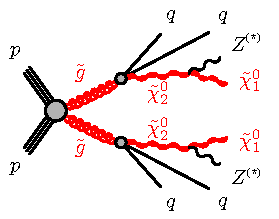
\includegraphics[width=.9\linewidth]{figures/theory/gogo-qqqqZZN1N1.pdf}
\caption{Feynman diagram of the decay considered in the simplified models used in the analysis presented in \autoref{part:search}.}
\label{fig:simpmodel}
\end{figure}
\end{centering}

Using this simplified model, the masses of the particles can be tuned directly. This is very helpful for the generation of \ac{MC}, discussed in \autoref{sec:MC_gen}, because a ``grid'' of different mass points of the important sparticles involved in the decay can be generated, allowing analyzers to make predictions of likely signals, and to exclude the simplified models as a function of the mass of the sparticles in the case that no anomalies are seen. 

\section{Monte Carlo Generators}
\label{sec:MC_gen}

The complex events of the \ac{LHC} are difficult to model, but modeling them is crucial to analyzers' understanding of \ac{SM} backgrounds and potential signals. To simplify the modeling process, particle interactions are broken down into very small steps, each with associated probabilities of various outcomes. This modeling method is called \acf{MC}, and, at the \ac{LHC} it is broken into several larger steps which are each handled by different software. 

The first step, discussed in \autoref{sec:pp_collisions}, is to determine the energies of the initial particles in a collision, which provided by several different \ac{PDF} sets. 


